\documentclass[12pt]{report}
\usepackage[utf8]{inputenc}
\usepackage{polski}
\usepackage[polish]{babel}
\usepackage[a4paper,width=170mm,top=25mm,bottom=25mm,bindingoffset=6mm]{geometry}
\usepackage{graphicx}
\usepackage{listings}
\usepackage{xcolor}
\usepackage{setspace}
\usepackage{biblatex}
\addbibresource{references.bib}
\graphicspath{{./images/}}

\newcommand{\makeTitlePage}{
    \begin{titlepage}
        \begin{center}
            
\includegraphics[width=0.4\textwidth]{../images/agh_logo.png} \\
            \large{
                Akademia Górniczo-Hutnicza im. Stanisława Staszica w Krakowie \\
                Wydział Informatyki, Elektroniki i Telekomunikacji \\
                Instytut Informatyki \\
            }
            \vspace{1.5cm}
            \textbf{\LARGE{Języki formalne i kompilatory}} \\
            \vspace{1.0cm}
            \Huge
            \LARGE{Projekt zaliczeniowy} \\
            \vspace{1.0cm}
            \textit{\textbf{Translator języka \LaTeX \space do HTML}} \\
            \vfill
            \Large{\textbf{Bartosz Kordek Grzegorz Zacharski}} \\
            \vspace{0.5cm}
            \large{Informatyka} \\
            \vspace{0.3cm}
            \large{Studia niestacjonarne} \\
            \vspace{0.7cm}
            \large{Kraków, 2021}
        \end{center}
        \normalsize
    \end{titlepage}
}

\definecolor{codegreen}{rgb}{0,0.6,0}
\definecolor{codegray}{rgb}{0.5,0.5,0.5}
\definecolor{codepurple}{rgb}{0.58,0,0.82}
\definecolor{backcolour}{rgb}{0.96,0.96,0.96}

\lstdefinestyle{mystyle}{
    backgroundcolor=\color{backcolour},   
    commentstyle=\color{codegreen},
    keywordstyle=\color{magenta},
    numberstyle=\tiny\color{codegray},
    stringstyle=\color{codepurple},
    basicstyle=\ttfamily\footnotesize,
    breakatwhitespace=false,         
    breaklines=true,                 
    captionpos=b,                    
    keepspaces=true,                 
    numbers=left,                    
    numbersep=5pt,                  
    showspaces=false,                
    showstringspaces=false,
    showtabs=false,                  
    tabsize=2
}
\lstset{style=mystyle}

\begin{document}
    \makeTitlePage

    \onehalfspacing

    \tableofcontents

    \chapter{Wstęp}

Celem projektu było zaimplementowanie translatora języka LaTeX do HTML. W tym celu skorzystaliśmy z gotowej biblioteki do parsowania
PLY w języku Python. Kod odpowiadający za wykonanie translacji podzieliliśmy na dwie części: parser i lekser.

    \chapter{Specyfikacja gramatyki}

\section{Tekst}

\section{Formatowanie tekstu}
    fasfasfa

\section{Tabela}

\section{Wyliczenie}

\section{Grafika}

\section{Hiperłącze}

\section{Sekcja, podsekcja, podpodsekcja}


% TODO 
% specyfikację gramatyki języka w notacji wybranego przez siebie narzędzia 
% wzorowane na Rozdziale 1 oraz Dodatku „Przewodnik języka C” (Sekcja „Gramatyka”) 
% książki „Język C”, B. Kernighan, D. Ritchie.

    \chapter{Gramatyka}

\section{Lexer}
Na listingu \ref{analiza-leksykalna-tokeny} zostały przedstawione tokeny obsługiwane przez nasz translator.

\begin{lstlisting}[language={Python}, caption={Analiza leksykalna - podział na tokeny}, label={analiza-leksykalna-tokeny}]
    tokens = (
        'AUTHOR',
        'BEGIN_DOCUMENT',
        'BEGIN_OLIST',
        'BEGIN_ULIST',
        'BEGIN_TABULAR',
        'BOLD',
        'CENTERLINE',
        'CHAPTER',
        'COLUMN_DIVIDER',
        'COLUMN_PATTERN_BORDERLESS',
        'COLUMN_PATTERN_BORDERED',
        'DOCUMENTCLASS',
        'END_DOCUMENT',
        'END_OLIST',
        'END_ULIST',
        'END_TABULAR',
        'GRAPHICS_PATH',
        'HLINE',
        'INCLUDE_GRAPHICS',
        'ITALIC',
        'ITEM',
        'LBRACE',
        'NEW_LINE',
        'NULL',
        'PARAGRAPH',
        'RBRACE',
        'ROW_END',
        'SECTION',
        'SUBSECTION',
        'SUBSUBSECTION',
        'TEXT',
        'TITLE',
        'UNDERLINE',
        'URL',
        'USE_PACKAGE',
    )
\end{lstlisting}

Tokeny na listingu \ref{analiza-leksykalna-tokeny} odpowiadają następującym wyrażeniom regularnym 
przedstawionym na listingu \ref{analiza-leksykalna-wyrazenia}:

\begin{lstlisting}[language={Python}, caption={Analiza leksykalna - wyrażenia regularne}, label={analiza-leksykalna-wyrazenia}]
    t_AUTHOR = r'\\author'
    t_BEGIN_DOCUMENT = r'\\begin\{document\}'
    t_BEGIN_OLIST = r'\\begin\{enumerate\}'
    t_BEGIN_ULIST = r'\\begin\{itemize\}'
    t_BEGIN_TABULAR = r'\\begin\{tabular\}'
    t_BOLD = r'\\textbf'
    t_CENTERLINE = r'\\centerline'
    t_CHAPTER = r'\\chapter'
    t_COLUMN_DIVIDER = r'&'
    t_COLUMN_PATTERN_BORDERLESS = r'\{[lcr](\s[lcr])*\}'
    t_COLUMN_PATTERN_BORDERED = r'\{(\|\s[lcr]\s)+\|\}'
    t_DOCUMENTCLASS = r'\\documentclass.*'
    t_END_DOCUMENT = r'\\end\{document\}'
    t_END_OLIST = r'\\end\{enumerate\}'
    t_END_ULIST = r'\\end\{itemize\}'
    t_END_TABULAR = r'\\end\{tabular\}'
    t_GRAPHICS_PATH = r'\\graphicspath'
    t_INCLUDE_GRAPHICS = r'\\includegraphics'
    t_ITALIC = r'\\textit'
    t_ITEM = r'\\item'
    t_LBRACE = r'\{'
    t_NEW_LINE = r'\\newline'
    t_NULL = r'\0'
    t_PARAGRAPH = r'\\paragraph'
    t_RBRACE = r'\}'
    t_ROW_END = r'\\\\'
    t_SECTION = r'\\section'
    t_SUBSECTION = r'\\subsection'
    t_SUBSUBSECTION = r'\\subsubsection'
    t_TEXT = r'[\w\d\.,!?@#/\'\"<>\(\)\-+=\/^\*:;|\[\]]+'
    t_TITLE = r'\\title'
    t_UNDERLINE = r'\\underline'
    t_URL = r'\\url'
    t_USE_PACKAGE = r'\\usepackage.*'
\end{lstlisting}

Definicje tokenów nowej linii, komentarza, błędów oraz tokenów ignorowanych zostały przedstawione na listingu \ref{analiza-leksykalna-pozostale}.

\begin{lstlisting}[language={Python}, caption={Analiza leksykalna - pozostałe tokeny}, label={analiza-leksykalna-pozostale}]
    def t_newline(self, t):
        r'\n+'
        t.lexer.lineno += t.value.count("\n")

    def t_comment(self, t):
        r'%.*\n'
        pass

    def t_hline(self, t):
        r'\\hline'
        pass

    t_ignore = ' '

    def t_error(self, t):
        print("Illegal character '%s'" % t.value[0])
        t.lexer.skip(1)
\end{lstlisting}

Należy zauważyć, że cała zawartość między znacznikiem "\textbf{\%}" w formacie \LaTeX, odpowiadającemu początkowi komentarza, do nowej linii, 
zostaje pominięta.

\section{Parser}

Każdy z dokumentów HTML'a musi zawierać znaczniki typowe dla tego formatu, których nie znajdziemy w dokumentach \LaTeX. Są to: \textbf{\textit{html}},
\textbf{\textit{head}} oraz \textbf{\textit{body}}. Jako odpowienik sekcji \textbf{\textit{head}} przyjęliśmy sekcję preambuly w której 
znajdują się między innymi takie polecenia jak \textit{usepackage}. Natomiast jak odpowiednik sekcji \textbf{\textit{body}} odpowiada fragment kodu 
\LaTeX \space objęty poleceniami \textit{begin\{document\}} oraz \textit{end\{document\}}.

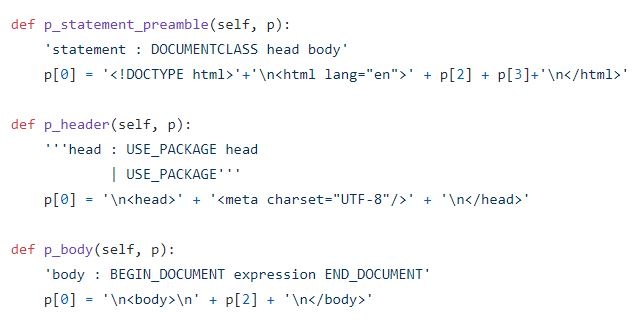
\includegraphics{preamble.JPG}

\subsection{Obsługa tekstu}

\begin{lstlisting}[language={Python}, caption={Gramatyka - tekst}, label={gramatyka-tekst}]
    def p_expression_text(self, p):
        '''expression : TEXT expression
                      | TEXT'''
        if len(p) == 3:
            p[0] = p[1] + " " + p[2]
        else:
            p[0] = p[1]
\end{lstlisting}

\subsection{Formatowanie tekstu}

Nasz translator umożliwia pogrubienie, kursywę, podkreślenie, wyśrodkowanie tekstu oraz utworzenie paragrafu. 
Możliwe jest mieszanie stylów formatowania, np. pogrubienie z podkreśleniem. 
Według nowych zaleceń, do pogrubienia tekstu w HTML'u powinno się stosować znacznik
\textit{$<$strong$>$}, a do kursywy \textit{$<$em$>$}.

\begin{lstlisting}[language={Python}, caption={Formatowanie - pogrubienie, kursywa, podkreślenie, wyśrodkowanie tekstu}, label={gramatyka-pogrubienie-kursywa}]
    def p_expression_bold(self, p):
        '''expression : BOLD LBRACE expression RBRACE expression
                      | BOLD LBRACE expression RBRACE'''
        if len(p) == 6:
            p[0] = '<strong>' + p[3] + '</strong>' + p[5]
        else:
            p[0] = '<strong>' + p[3] + '</strong>'

    def p_expression_italic(self, p):
        '''expression : ITALIC LBRACE expression RBRACE expression
                      | ITALIC LBRACE expression RBRACE'''
        if len(p) == 6:
            p[0] = '<em>' + p[3] + '</em>' + p[5]
        else:
            p[0] = '<em>' + p[3] + '</em>'

    def p_expression_underline(self, p):
        '''expression : UNDERLINE LBRACE expression RBRACE expression
                      | UNDERLINE LBRACE expression RBRACE'''
        if len(p) == 6:
            p[0] = '<u>' + p[3] + '</u>' + p[5]
        else:
            p[0] = '<u>' + p[3] + '</u>'

    def p_expression_centerline(self, p):
        '''expression : CENTERLINE LBRACE expression RBRACE expression
                      | CENTERLINE LBRACE expression RBRACE'''
        if len(p) == 6:
            p[0] = '<center>' + p[3] + '</center>' + p[5]
        else:
            p[0] = '<center>' + p[3] + '</center>'

    def p_expression_paragraph(self, p):
        '''expression : PARAGRAPH LBRACE expression RBRACE expression
                      | PARAGRAPH LBRACE expression RBRACE'''
        if len(p) == 6:
            p[0] = '<p>' + p[3] + '</p>' + p[5]
        else:
            p[0] = '<p>' + p[3] + '</p>'
\end{lstlisting}

Kolejną funkcjonalnością jest możliwość obsługi rozdziałów, sekcji i podsekcji parsując 
znaczniki \textit{chapter}, \textit{section}, \textit{subsection} oraz \textit{subsubsection}.

\begin{lstlisting}[language={Python}, caption={Rozdziały, sekcje i podsekcje}, label={gramatyka-sekcje-podsekcje}]
    def p_expression_chapter(self, p):
        '''expression : CHAPTER LBRACE expression RBRACE expression
                      | CHAPTER LBRACE expression RBRACE'''
        if len(p) == 6:
            p[0] = '<h1>' + p[3] + '</h1>' + p[5]
        else:
            p[0] = '<h1>' + p[3] + '</h1>'

    def p_expression_section(self, p):
        '''expression : SECTION LBRACE expression RBRACE expression
                      | SECTION LBRACE expression RBRACE'''
        if len(p) == 6:
            p[0] = '<h2>' + p[3] + '</h2>' + p[5]
        else:
            p[0] = '<h2>' + p[3] + '</h2>'

    def p_expression_subsection(self, p):
        '''expression : SUBSECTION LBRACE expression RBRACE expression
                      | SUBSECTION LBRACE expression RBRACE'''
        if len(p) == 6:
            p[0] = '<h3>' + p[3] + '</h3>' + p[5]
        else:
            p[0] = '<h3>' + p[3] + '</h3>'

    def p_expression_subsubsection(self, p):
        '''expression : SUBSUBSECTION LBRACE expression RBRACE expression
                      | SUBSUBSECTION LBRACE expression RBRACE'''
        if len(p) == 6:
            p[0] = '<h4>' + p[3] + '</h4>' + p[5]
        else:
            p[0] = '<h4>' + p[3] + '</h4>'
\end{lstlisting}

Przejście do nowej linii (hard break) jest obsłużone poleceniem \textit{newline}.

\begin{lstlisting}[language={Python}, caption={Nowa linia}, label={gramatyka-nowa-linia}]
    def p_expression_newline(self, p):
        '''expression : NEW_LINE expression
                      | NEW_LINE'''
        if len(p) == 3:
            p[0] = '<br/>' + p[2]
        else:
            p[0] = p[1]
\end{lstlisting}

Translator parsuje również znacznik \textit{title} odpowiadający za utworzenie tytułu.

\begin{lstlisting}[language={Python}, caption={Tytuł}, label={gramatyka-tyti}]
    def p_title(self, p):
        'expression : TITLE LBRACE TEXT RBRACE'
        p[0] = '<i>' + p[3] + '</i>'
\end{lstlisting}

\subsection{Tabela}

\subsubsection{Z obramowaniem}

\begin{lstlisting}[language={Python}, caption={Tabela z obramowaniem}, label={gramatyka-tekst}]
    def p_expression_table_bordered(self, p):
        '''expression : BEGIN_TABULAR COLUMN_PATTERN_BORDERED tablerowbordered END_TABULAR expression | BEGIN_TABULAR COLUMN_PATTERN_BORDERED tablerowbordered END_TABULAR'''
        if len(p) == 6:
            p[0] = '<table style="border: 1px solid black; border-collapse: collapse;">' + p[3] + '</table>' + p[5]
        else:
            p[0] = '<table style="border: 1px solid black; border-collapse: collapse;">' + p[3] + '</table>'

    def p_tablerowbordered(self, p):
        '''tablerowbordered : tablecolumnbordered ROW_END tablerowbordered | tablecolumnbordered'''
        if len(p) == 4:
            p[0] = '<tr>' + p[1] + '</tr>' + p[3]
        else:
            p[0] = '<tr>' + p[1] + '</tr>'

    def p_tablecolumnbordered(self, p):
        '''tablecolumnbordered : expression COLUMN_DIVIDER tablecolumnbordered | expression'''
        if len(p) == 4:
            p[0] = '<td style="border: 1px solid black; border-collapse: collapse;">' + p[1] + '</td>' + p[3]
        else:
            p[0] = '<td style="border: 1px solid black; border-collapse: collapse;">' + p[1] + '</td>'
\end{lstlisting}

\subsubsection{Bez obramowania}

\begin{lstlisting}[language={Python}, caption={Tabela bez obramowania}, label={gramatyka-tekst} ]
    def p_expression_table_borderless(self, p):
        '''expression : BEGIN_TABULAR COLUMN_PATTERN_BORDERLESS tablerowborderless END_TABULAR expression | BEGIN_TABULAR COLUMN_PATTERN_BORDERLESS tablerowborderless END_TABULAR'''
        if len(p) == 6:
            p[0] = '<table>' + p[3] + '</table>' + p[5]
        else:
            p[0] = '<table>' + p[3] + '</table>'

    def p_tablerowborderless(self, p):
        '''tablerowborderless : tablecolumnborderless ROW_END tablerowborderless | tablecolumnborderless'''
        if len(p) == 4:
            p[0] = '<tr>' + p[1] + '</tr>' + p[3]
        else:
            p[0] = '<tr>' + p[1] + '</tr>'

    def p_tablecolumnborderless(self, p):
        '''tablecolumnborderless : expression COLUMN_DIVIDER tablecolumnborderless | expression'''
        if len(p) == 4:
            p[0] = '<td>' + p[1] + '</td>' + p[3]
        else:
            p[0] = '<td>' + p[1] + '</td>'
\end{lstlisting}

\subsection{Wyliczenie}

Konstrukcja parsera wyliczeń umożliwia wykonywanie zagnieżdżeń.

\subsubsection{Uporządkowane}

\begin{lstlisting}[language={Python}, caption={Gramatyka - tabela}, label={gramatyka-tekst} ]
    def p_expression_ordered_list(self, p):
        '''expression : BEGIN_OLIST listitems END_OLIST expression
                      | BEGIN_OLIST listitems END_OLIST'''
        if len(p) == 5:
            p[0] = '\n<ol>' + p[2] + '\n</ol>' + p[4]
        else:
            p[0] = '\n<ol>' + p[2] + '\n</ol>'
\end{lstlisting}

\subsubsection{Nieuporządkowane}

\begin{lstlisting}[language={Python}, caption={Gramatyka - tabela}, label={gramatyka-tekst} ]
    def p_expression_unordered_list(self, p):
        '''expression : BEGIN_ULIST listitems END_ULIST expression
                      | BEGIN_ULIST listitems END_ULIST'''
        if len(p) == 5:
            p[0] = '\n<ul>' + p[2] + '\n</ul>' + p[4]
        else:
            p[0] = '\n<ul>' + p[2] + '\n</ul>'
\end{lstlisting}

\subsection{Grafika}

Umieszcznie grafiki jest możliwe dzięki znacznikowi \textit{includegraphics} w \LaTeX, który jest parsowany na znacznik 
\textit{$<$img$>$} w HTML, gdzie atrybut \textit{src} stanowi ścieżka do pliku umieszczona w nawiasach 
wąsatych w dokumencie \LaTeX.

\begin{lstlisting}[language={Python}, caption={Grafika}, label={gramatyka-tekst} ]
    def p_expression_includegraphics(self, p):
        '''expression : INCLUDE_GRAPHICS TEXT LBRACE expression RBRACE expression 
                      | INCLUDE_GRAPHICS LBRACE expression RBRACE expression 
                      | INCLUDE_GRAPHICS LBRACE expression RBRACE'''
        if len(p) == 7:
            attributes = p[2][1:-1]
            p[0] = '''<img src="''' + p[4] + '''"''' + attributes + '''>''' + p[6]
        elif len(p) == 6:
            p[0] = '''<img src="''' + p[3] + '''">''' + p[5]
        else:
            p[0] = '''<img src="''' + p[3] + '''">'''
\end{lstlisting}

\subsection{Hiperłącze}

Zamieszczenie hiperłącza w formacie \LaTeX jest możliwe dzięki znacznikowi \textit{url}, 
zawierającego w nawiasach wąsatych adres do strony.
Parsowanny jest on na HTML'owy znacznik \textit{$<$a$>$} z atrybutem \textit{href} zawierającego adres.

\begin{lstlisting}[language={Python}, caption={Hiperłącze}, label={gramatyka-hiperlacze} ]
    def p_expression_url(self, p):
        '''expression : URL LBRACE expression RBRACE expression
                      | URL LBRACE expression RBRACE'''
        if len(p) == 6:
            p[0] = '<a href=' + p[3] + '>' + p[3] + '</a>' + p[5]
        else:
            p[0] = '<a href=' + p[3] + '>' + p[3] + '</a>'
\end{lstlisting}

    \chapter{Uzasadnienie wyboru generatora}

Ze względu języki programowania rozważaliśmy generatory parserów, do wykorzystania których moglibyśmy użyć języków Java lub Python. 
Głównie skupiliśmy się na PLY i SLY z Pythona oraz JavaCC. Ostatecznie wybraliśmy generator parserów PLY, ze względu na powszechność 
stosowania, dostępność i jakość dokumentacji. Ponadto chcieliśmy również nabrać więszego doświadczenia w stosowaniu języka Python.

    \input{chapters/opis_problemów.tex}

    \lstlistoflistings

    \printbibliography
    
\end{document}